\section{Pretplata}
Predstavlja jedan način podrške časopisa od strane čitalaca. Jedna od prednosti je dobijanje izdanja po povoljnijoj ceni u poređenju sa kupovanjem pojedninačnih primeraka. 

Druga pogodnost je da će časopis biti dostavljen na kućnu adresu čitaoca. Takođe, ne postoji bojazan da bi čitaloci mogli da zaborave da kupe mesečno izdanje časopisa usled nedostatka vremena ili odsustva.

\subsection{Osmišljanje modela pretplate}
\begin{description}
\item [Opis] Menadžment razmatra različite tipove pretplate sa stanovišta perioda i cene pretplate.
\item [Učesnici] Menadžment.
\item [Preduslov] Nema.
\item [Postuslov] Definisani jedan ili više modela pretplate.
\end{description}
\subsubsection{Glavni tok}
Menadžment postavlja okvire cene i perioda nad kojima se vrši pretplata. Uzimaju se u obzir uobičajeni vremenski periodi na koje bi se davala pretplata(npr. 6m, 1g, 2g) kao i odgovarajuća cena.
Ukoliko se časopis ne izdaje u intervalima od jednog meseca, pretplata se zasniva na broju primeraka. Menadžment dalje odlučuje za svaki predloženi model pretplate dodatne pogodnosti kojima će nagraditi pretplatnike.
Vrši se odabir jednog ili više predloženih modela pretplate.

\subsection{Ugovaranje pretplate}
\begin{description}
\item [Opis] Čitalac kontaktira menadžment časopisa radi pretplate.
\item [Učesnici] Čitalac, menadžment.
\item [Ulaz] Kontakt čitaoca.
\item [Izlaz] Izvršena pretplata.
\item [Preduslov] Časopis ima definisane modele pretplate.
\item [Postuslov] Čitalac se uspešno pretplatio.
\end{description}
\subsubsection{Glavni tok}
Menadžment pre isporuke novog izdanja na prodajna mesta kontaktira distributera. Pre toga dohvata informacije o adresama stanovanja pretplatnika i prosleđuje ih distributeru. 
Distributer, zajedno sa primercima časopisa i podacima o adresama vrši isporuku.
\subsubsection{Alternativni tok}
Ukoliko čitalac iz određenih okolnosti odluči da prekine pretplatu, to saopštava menadžmentu i vrši se delimični povraćaj novca.

\begin{figure}[ht]
    \centering
    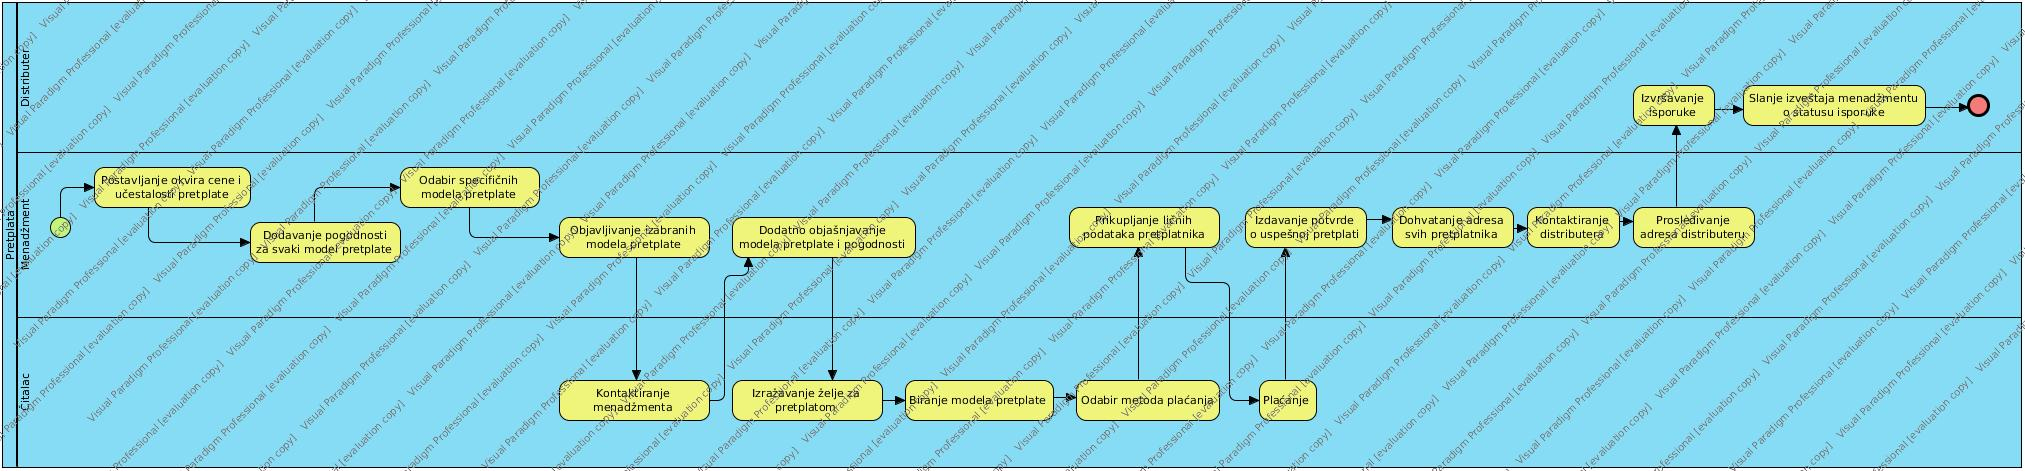
\includegraphics[width=0.9\textheight, angle=90]{slike/pretplata}
    \caption{BPMN dijagram - Pretplata}
    \label{pretplata}
\end{figure}

\subsection{Distribucija časopisa pretplatnicima}
\begin{description}
\item [Opis] Menadžment organizuje dostavu časopisa pretplatnicima.
\item [Učesnici] Menadžment, distributer.
\item [Preduslov] Primerci časopisa za isporuku su ištampani.
\item [Postuslov] Časopis dostavljen na krajnju adresu čitalaca.
\end{description}
\subsubsection{Glavni tok}
Menadžment pre isporuke novog izdanja na prodajna mesta kontaktira distributera. Pre toga dohvata informacije o adresama stanovanja pretplatnika i prosleđuje ih distributeru. Distributer, zajedno sa primercima časopisa i podacima o adresama vrši isporuku.
Po uspešno izvršenoj isporuci javlja menadžmentu da li je isporuka uspešno izvršena, kako bi eventualno pretplatnici bili obavešteni o mogućim komplikacijama.


